%===============================================================================
% $Id: ifacconf.tex 19 2011-10-27 09:32:13Z jpuente $  
% Template for IFAC meeting papers
% Copyright (c) 2007-2008 International Federation of Automatic Control
%===============================================================================
\documentclass[a4paper]{ifacconf}

\usepackage[utf8]{inputenc}
\usepackage{fourier} 
\usepackage{array}
\usepackage{makecell}
\usepackage{graphicx,amsmath,url}      % include this line if your document contains figures
\usepackage[round]{natbib}             % required for bibliography
%===============================================================================


% ===============================================================
% Choose the language of the manuscript.
% If in English, choose 
% \def\portugues{0} 
%
% If in Portuguese or Spanish, choose
% \def\portugues{1} 
%
% Note that, if you are writing in Spanish, you need additional 
% adjusts in some parts of the text, which have been put in Portuguese only.
\def\portugues{1} 
% ===============================================================

% If the above line is commented, it is assumed manuscript in English:
\ifx\portugues\undefined
\def\portugues{0}
\fi


\if\portugues0
   \usepackage[english]{babel}
  \else
   \usepackage[spanish,brazil,english]{babel}
\fi

  

\usepackage[T1]{fontenc}
%\usepackage{inputenc}

\usepackage[utf8]{inputenc}

\usepackage{ae}


\if\portugues1
% =====================================================================
% =====================================================================
% If the manuscript is in Spanish, please change the texts adequatelly.
% You may also add other definitions in this part.
 \newtheorem{teorema}[thm]{{\em Teorema}}{ }
 \newtheorem{lema}[thm]{{\em Lema}}{ }
 \newtheorem{corolario}[thm]{{\em Corolário}}{ }
 \newenvironment{prova}{{\bf Prova.}}{ }
% ===============================================================
\fi

\begin{document}
	
	
\if\portugues1

% =====================================================================
% =====================================================================
% USE THIS PART IF THE TEXT IS IN PORTUGUES OR SPANISH
% =====================================================================
% If the manuscript is in Spanish, please change the texts adequately.
% =====================================================================
% 
\selectlanguage{brazil}
	
\begin{frontmatter}

\title{Uma Abordagem de Aprendizado Online para o Seguimento de Trajetórias usando Robôs não Holonômicos} 
% Title, preferably not more than 10 words.

%\thanksref{footnoteinfo}
%\thanks[footnoteinfo]{Reconhecimento do suporte financeiro deve vir nesta nota de rodapé.}


\author[First]{Mateus Sousa Franco}, 
\author[First]{Sérgio R. Barros dos Santos}
\author[First]{Fábio Augusto Faria}

\address[First]{Instituto de Ciência e Tecnologia, Universidade Federal de São Paulo, SP, (e-mail: mateus.franco@unifesp.br e sergio.ronaldo@unifesp.br).}


\selectlanguage{english}
\renewcommand{\abstractname}{{\bf Abstract:~}}
\begin{abstract}                % Abstract of not more than 250 words.
This study investigate the implementation of a Reinforcement Learning (RL) method to derivate control laws of a non-holonimic robot considering the coupling and non-linearty of the system. The controller is online derivated from the interaction between the agent and the unknown environment implementing a Q-learning based approach to find the best action to be taken maximizing rewards along attempts to follow the trajectory. The presented study cases show that the learned controllers were capable of efficiently follow different trajectories considering the variation of translation and rotation speeds and maximizing the reward amount over iteractions for two different learning process configurations.  


\vskip 1mm% não altere esse espaçamento
\selectlanguage{brazil}
{\noindent \bf Resumo}:  
Este artigo investiga a aplicação de um método de Aprendizado por Reforço (RL) para derivar as leis de controle de um robôs não holonômico, considerando o acoplamento e a não-linearidade do sistema. Os controladores são derivados \emph{on-line} através da interação entre o agente real e o ambiente desconhecido, usando uma abordagem baseada no algoritmo \emph{Q-Learning}, que visa descobrir qual a melhor ação a ser tomada pelo agente, de modo a maximizar as recompensas recebidas em cada tentativa de execução do seguimento da trajetória desejada. Resultados experimentais mostraram que os controladores aprendidos são capazes de realizar o seguimento de diferentes trajetórias, de forma eficiente, levando em conta a variação das velocidades de translação e de rotação do robô maximizando o valor da recompensa ao longo das iterações, conforme apresentado nos estudos de caso.


\end{abstract}

\selectlanguage{english}


\begin{keyword}
Reinforcement Learning; Online Learning; Q-learning; Line-follower; PID Controller; Computer Vision;

\vskip 1mm% não altere esse espaçamento
\selectlanguage{brazil}
{\noindent\it Palavras-chaves:} Aprendizado por Reforço; Aprendizado Online; Q-learning; Seguidor de Linha; Controlador PID; Visão Computacional
\end{keyword}


\selectlanguage{brazil}


\end{frontmatter}
\else
% ===============================================================
% ===============================================================
% USE THIS PART IF THE TEXT IS IN ENGLISH
% ===============================================================
% ===============================================================
% 

\begin{frontmatter}

\title{Style for SBA Conferences \& Symposia: Use Title Case for
  Paper Title\thanksref{footnoteinfo}} 
% Title, preferably not more than 10 words.

\thanks[footnoteinfo]{Sponsor and financial support acknowledgment
goes here. Paper titles should be written in uppercase and lowercase
letters, not all uppercase.}

\author[First]{First A. Author} 
\author[Second]{Second B. Author, Jr.} 
\author[Third]{Third C. Author}


\address[First]{Faculdade de Engenharia Elétrica, Universidade do Triângulo, MG, (e-mail: autor1@faceg@univt.br).}
\address[Second]{Faculdade de Engenharia de Controle \& Automação, Universidade do Futuro, RJ (e-mail: autor2@feca.unifutu.rj)}
\address[Third]{Electrical Engineering Department, 
   Seoul National University, Seoul, Korea, (e-mail: author3@snu.ac.kr)}
   
\renewcommand{\abstractname}{{\bf Abstract:~}}   
   
\begin{abstract}                % Abstract of not more than 250 words.
These instructions give you guidelines for preparing papers for IFAC
technical meetings. Please use this document as a template to prepare
your manuscript. For submission guidelines, follow instructions on
paper submission system as well as the event website.
\end{abstract}

\begin{keyword}
Five to ten keywords, preferably chosen from the IFAC keyword list.
\end{keyword}

\end{frontmatter}
\fi


%*********************************************************************************************
% SEÇÃO 1
%*********************************************************************************************
\section{Introdução}

As técnicas clássicas de projeto de controladores envolvem a obtenção de um modelo matemático do sistema a ser controlado, que nada mais é do que um conjunto de expressões que descrevem e modelam o seu comportamento. Esta etapa tende a ter uma complexidade que varia de acordo com o tipo de sistema e com as condições estabelecidas para a derivação dos modelos, podendo levar a modelos matemáticos extremamente complexos, mesmo que lineares, e não necessariamente precisos. 
%A complexidade de modelos não-lineares tende a ser maior, entretanto, qualquer sistema não-linear pode ser linearizado para uma certa condição de operação, que é definida durante a linearização.

Um tipo de controlador amplamente utilizado devido à sua simplicidade de otimização e implementação é o controlador Proporcional-Integral-Derivativo (PID). Este controlador gera uma saída de controle proporcional ao erro entre o estado desejado e o estado atual (ganho proporcional), levando em consideração também a taxa de variação do erro (ganho derivativo) e o erro acumulado ao longo do tempo (ganho integral). O PID é um controlador geralmente empregado em sistemas lineares, porém também pode ser utilizado em sistemas não-lineares \citep{nonLinearPID} desde que algumas condições sejam estabelecidas durante a etapa de projeto do sistema de controle. \citep{pid_autotune_relay, pid_engine_tuning,embarcados_pid_1}.

O \emph{Reinforcement Learning} (RL), do inglês, Aprendizado por Reforço, é definido como um método de otimização para aplicações onde se deseja solucionar uma variedade de problemas de planejamento e controle da execução de tarefas, em que os modelos dos sistemas não estão disponíveis a priori. A partir da interação direta com ambiente, o agente aprende estratégias de controle adaptáveis a diferentes situações encontradas, através de recompensas, na forma de reforços positivos ou negativos, sinalizando ao agente se a ação tomada foi correta ou incorreta, respectivamente. O objetivo do agente sempre será acumular o máximo de reforço positivo possível durante a exploração do ambiente aleatório e desconhecido \citep{ql_pid_robotics,intro_to_rl,rl_rob_survey,ql_pid_robotics}.

Este tipo de abordagem possui um grande potencial no âmbito da robótica móvel, uma vez que robôs móveis são classificados como sistemas não-lineares, cujo comportamento possui um elevado acoplamento e grau de incerteza associada à determinação dos estados, que são obtidos através da amostragem de sensores. Uma modelagem matemática rigorosa deste sistema geralmente leva a expressões e soluções complexas, de modo que um controlador simples como o PID não funcione de forma adequada. Neste contexto, uma vantagem de realizar o aprendizado diretamente no robô real é que os controladores aprendidos levam em consideração o acoplamento e a não-linearidade do sistema, sendo esses fatores usualmente desconsiderados em projeto de controladores, em virtude das simplificações adotadas \citep{ql_pid_robotics}.

O objetivo deste trabalho é implementar um algoritmo de controle não linear baseado na abordagem \textit{online} de RL, que seja capaz de se adaptar às diferentes condições de operação do agente durante a realização do seguimento de trajetórias. A partir da interação entre o agente e o ambiente, o algoritmo RL busca encontrar um controlador que seja capaz de executar o trajeto desejado com precisão e eficiência, para diferentes velocidades de translação e de rotação. 

%O aprendizado do sistema de controle é realizado diretamente no robô real, assim, tanto o algoritmo de RL quanto as malhas de controle são implementadas no computador embarcado. Sensores infravermelhos e um sistema de visão são usados para determinar o estado atual do agente no ambiente. Usando as informações fornecidas a respeito dos estados e conhecendo as ações realizadas, é estimado o reforço aplicado ao agente em cada episódio. 

O aprendizado do sistema de controle é realizado diretamente no robô real, ou seja, o algoritmo de RL é implementadas diretamente no computador embarcado, que também possui um sistema de visão para aferir o estado do agente a partir do qual é calculado o sinal de reforço aplicado a cada episódio.

O artigo está organizado da seguinte forma: Na Seção 2, é apresentada a formulação do problema assim como uma descrição do robô e da estrutura de controle baseada em RL. A Seção 3 é dedicada à apresentação da estratégia proposta para o processo de aprendizagem online do sistema de controle para rastreamento de diferentes trajetórias. Em seguida, apresentamos o ambiente experimental utilizado para o treinamento do sistema considerando diferentes velocidade de translação e de rotação na Seção 4. Na Seção 5, apresentamos os resultados obtidos durante a fase de aprendizagem do rastreamento de trajetórias. As conclusões são apresentadas na Seção 6.

%*********************************************************************************************
% SEÇÃO 2
%*********************************************************************************************
\section{Preliminares}
%A otimização da trajetória do robô é um dos problemas que podem ser resolvidos no caso do robô seguidor de linha aplicando o RL. Quanto menos o robô se desvia da trajetória definida pela linha, menor é o erro de posição entre o robô e a linha e, consequentemente, menor o tempo que o robô gasta para percorrer o circuito. Neste caso, por meio das interações, o RL irá aprender qual é a melhor combinação de velocidades de rotação dos motores para que o robô se mantenha o mais próximo possível da linha, condição de maiores recompensas.

%O motor de corrente contínua utilizado na maioria dos robôs se trata de um sistema não-linear, cuja modelagem rigorosa leva à expressões extremamente complexas. A otimização através do RL torna possível a obtenção de controladores ótimos e consequentemente um melhor controle de trajetória. No caso do controle de trajetória, o aprendizado por reforço permite que o robô aprenda a determinar sua melhor velocidade e direção a partir da posição relativa à linha, que é obtida através dos seus sensores.




%**********************
\subsection{Aprendizado por Reforço}

\emph{Reinforcement Learning} (RL) se trata de um método de \emph{Machine Learning} (ML), que permite ao agente (robô) descobrir, sem prévio conhecimento do ambiente, quais as melhores ações a serem tomadas de modo a maximizar a recompensa recebida em uma determinada tentativa de realizar a tarefa desejada \citep{intro_to_rl}. Este paradigma é diferente, por exemplo, do Aprendizado Supervisionado, que conta com um supervisor externo \citep{intro_to_rl,rl_rob_survey,ql_pid_robotics,ql_model}. O RL baseia-se em uma arquitetura formal que define a interação entre o agente e seu ambiente em termos dos estados, das ações e das recompensas (sinais de reforço).

De acordo com \citep{intro_to_rl}, um modelo de RL típico consiste em:
\begin{itemize}
  \item[•] Um conjunto $s$, discreto de estados do ambiente;
  \item[•] Um conjunto $a$, discreto de ações do agente;
  \item[•] Um conjunto de sinais de reforço $R$ normalmente \{0,1\} ou um número real.
\end{itemize}

O RL pode ser matematicamente formalizado utilizando o chamado \emph{Finite Markov Decision Process} (MDP), do inglês, Processo de Decisão Finito de Markov, que é uma formalização clássica de problemas de tomada de decisão onde a ação não influencia apenas as recompensas imediatas, mas também as situações, estados e recompensas futuras, onde a função de valor é estimada com base na ação e no estado atual \citep{ql_model,markov_tut}. 

A política define o modelo de comportamento do agente, ou seja, é o elemento que estabelece o mapeamento entre um dado estado e a ação executada pelo agente, baseado em probabilidades\citep{rl_rob_survey}. Se o agente está seguindo a política $\pi$ em um tempo $t$, então $\pi(a|s)$ é a probabilidade que $A_{t} = a$ se $S_{t} = s$. Dada uma política $\pi$, é possível definir formalmente a função ação-valor $q_{\pi}(a,s)$ como o valor de tomar uma ação $a$ em um estado $s$:

\begin{multline}
q_{\pi}(a,s) = \mathbb{E}[G_{t}|S_{t}=s,A_{t}=a] = \\ 
\mathbb{E}_{\pi}[\sum_{k=0}^{\infty} \gamma^k R_{t+k+1}|S_{t}=s,A_{t}=a], \forall s \in S, \forall a \in A(s)
\label{eq:actionValueFunc}
\end{multline}

Resolver a tarefa do RL significa encontrar a política ótima para o MDP, ou seja, encontrar a política que maximize a recompensa total ao longo do tempo. Considere uma política $\pi$ definida como melhor ou igual à política $\pi'$ para todos os estados. Sendo assim, pode-se inferir que $\pi \geq \pi' \Leftrightarrow v_{\pi}(s) \geq v_{\pi'}(s) \forall s \in S$. Sempre há uma política que é melhor ou igual às outras, esta é a política ótima $\pi_{*}$, que nem sempre é única. Todas as políticas ótimas compartilham a mesma função de estado-valor ótima, $v_{*}(s)$, e função de ação-valor ótima, $q_{*}(s,a)$ \citep{intro_to_rl}.
\begin{equation}
v_{*}(s) = \max_{\pi} v_{\pi}(s), \forall s \in S
\label{eq:bestStateValue}
\end{equation}
\begin{equation}
q_{*}(s,a) = \max_{\pi} q_{\pi}(s,a), \forall s \in S,\forall a \in A(s)
\label{eq:bestActionValue}
\end{equation}

Ainda é possível escrever $q_{*}(s,a)$ em termos de $v_{*}(s)$, de modo a obter uma função que fornece o retorno esperado para um par estado-ação seguindo a política ótima \citep{intro_to_rl}.

\begin{equation}
q_{*}(s,a) = \mathbb{E}[R_{t+1}+ \gamma .v_{*}(S_{t+1})|S_{t}=s,A_{t}=a]
\end{equation}

Especificamente, o \emph{Q-learning} pode ser usado para encontrar uma política de ações para qualquer MDP. Nessa abordagem, o agente (robô) aprende uma função de valor de ação (\emph{Q-function}), ou seja, uma função ótima $q_{*}$ de forma direta independente da política vigente, que define a utilidade esperada de tomar uma determinada ação ($a$) em um dado estado ($s$) \citep{Watkins92q-learning}. Assim, em cada iteração ou episódio, o algoritmo escolhe uma ação $a$ tal que a função $Q(S,A)$ seja maximizada.

\begin{equation}
Q(s,a) \leftarrow Q(s,a) + \alpha [R(s) + \gamma \max_{a} Q(s_1,a_1) - Q(s,a)]
\end{equation}

onde $R(s)$ o sinal de reforço imediato, $ Q(s_1,a_1)$ é o valor da função $Q$ referente ao próximo estado $s_1$ resultante da ação $a_1$, $\alpha$ é a taxa de aprendizagem e $\gamma$ refere-se ao parâmetro de desconto para as futuras recompensas no intervalo real [0,1).

%***************
\subsection{Modelagem Cinemática de Robôs não Holonômicos}

Considere o ponto $P$ centrado entre as rodas 1 (esquerda) e 2 (direita) que possuem um raio $r$ e estão localizadas à uma distância $l$ de $P$, com velocidades angulares $\dot{\varphi}_{1}$ e $\dot{\varphi}_{2}$ associadas. Uma vez que estes valores são conhecidos, é possível estabelecer o modelo matemático que define a cinemática dos movimentos de translação e rotação do robô em relação ao referencial inercial, que pode ser visto na Equação 2.6 \citep{intro_to_auto_robots}.

\begin{equation}
\dot{\xi_{I}} =
\begin{bmatrix}
\dot{x} \\
\dot{y} \\
\dot{\theta}
\end{bmatrix}=f(l,r,\theta,\dot{\varphi}_{1},\dot{\varphi}_{2}) 
\end{equation}

Suponha que o robô esteja alinhado ao eixo $X_{R}$ movendo-se no sentido positivo, ou seja, $\theta = 0^{\circ}$. Considere que a roda 1 está girando com velocidade angular $\dot{\varphi}_{1}$, enquanto a roda 2 permanece parada. A roda 1 irá transladar com uma velocidade tangencial $\dot{x}_{r1} = \dot{\varphi}_{1}r$ e fará com que o robô faça um movimento circular de raio $2l$ cujo centro de rotação é o ponto de contato da roda 2 com a superfície.

Como o ponto $P$ está exatamente na metade da distância entre a roda 1 e o centro de rotação, a sua velocidade de translação $\dot{x_{r}}$ é a metade da velocidade de translação da roda, conforme pode ser visto na Equação 2.7. Analogamente, pode-se adotar o mesmo raciocínio para o caso em que a roda 1 está parada e a roda 2 em movimento, dando origem à Equação 2.8.

\begin{equation}
\dot{x}_{r1}=\dfrac{r\dot{\varphi}_{1}}{2}
\end{equation}
\begin{equation}
\dot{x}_{r2}=\dfrac{r\dot{\varphi}_{2}}{2}
\end{equation}

A expressão que determina $\dot{x_{r}}$ é uma combinação dos efeitos causados pela rotação das duas rodas e pode ser obtida através da soma das duas expressões, conforme pode ser visto na Equação 2.9.
\begin{equation}
\dot{x_{r}} = \dot{x}_{r1} + \dot{x}_{r2}=\dfrac{r\dot{\varphi}_{1}}{2} + \dfrac{r\dot{\varphi}_{2}}{2}
\end{equation}

Agora suponha que as rodas possuem a mesma velocidade angular, porém sentidos de rotação opostos. Neste caso, o robô gira sobre ponto $P$, de forma estacionaria, de modo que $\dot{x}_{R}$ é nulo. O valor de $\dot{y}_{R}$ será sempre nulo, uma vez que nenhuma das rodas contribuiu com movimentos laterais.

Se a roda 1 (direita) gira num sentido que move o robô para frente enquanto a outra está parada, o ponto $P$ irá girar no sentido horário cujo centro de rotação é a roda parada. A velocidade angular de P pode ser calculada pela Equação 2.10.

\begin{equation}
\omega_{1} = \dfrac{r\dot{\varphi}_{1}}{2l}
\end{equation}

Uma situação análoga pode ser utilizada para derivar a expressão da velocidade angular de $P$ a partir da velocidade angular da roda 2 (esquerda). Basicamente apenas o sinal muda já que o sentido de rotação se inverte, conforme pode ser observado na Equação 2.11.

\begin{equation}
\omega_{2} = -\dfrac{r\dot{\varphi}_{2}}{2l}
\end{equation}

A combinação destas expressões individuais dá origem ao modelo cinemático do robô de duas rodas, dado pela equação 2.12.

\begin{equation}
\dot{\xi}_{I}=R(\theta)^{-1}
\begin{bmatrix}
\\ \dfrac{r\dot{\varphi}_{1}}{2}+\dfrac{r\dot{\varphi}_{2}}{2}\\
\\0 \\
\\ \dfrac{r\dot{\varphi}_{1}}{2l}-\dfrac{r\dot{\varphi}_{2}}{2l}
\end{bmatrix}
\end{equation}

onde $R(\theta)^{-1}$ refere-se a matriz de rotação ortogonal usada para transformação do sistema de coordenadas do robô para o sistema de coordenadas inercial. 

%*********************************************************************************************
% SEÇÃO 3
%*********************************************************************************************
\section{Desenvolvimento}

\subsection{Arquitetura Proposta}

%A \autoref{fig:gen_arq} mostra o diagrama de blocos de integração entre os módulos de \textit{Aprendizado por Reforço}, sistema de visão e controladores de velocidade e rotação.


%A Figura \ref{fig:blockDiagramFull} mostra o diagrama de blocos completo do sistema proposto, descrevendo a interconexão de cada bloco funcional. A Unidade de Servidor \textit{Web} (WU) e a Unidade de Visão Computacional e Aprendizado (CVLU), juntamente com seus quatro módulos: \textit{Q-learning}, Visão Computacional (CV), MCU (Comunicador) e o \textit{Integrator}, foram integradas através de um banco de dados e implementadas em um computador Raspberry Pi 3. A MCU, sendo composta pelos dois controladores de velocidade angular (\textit{Speed Controller 1 e 2}) e uma interface de comunicação com a CVLU foi implementada em um microcontrolador ATmega328. 

%A Unidade de Servidor \textit{Web}, implementa um servidor \textit{web} utilizando a linguagem Python, o \textit{module} Flask e um banco de dados gerenciado pelo MariaDB para disponibilizar informações relativas a processo de aprendizado em andamento e armazenar dados de processos anteriores, criando um histórico. Além disso, essa unidade também possibilita a visualização dos dados de forma remota e a partir de qualquer dispositivo. 

A Figura \ref{fig:blockDiagramFull} mostra o diagrama de blocos completo do sistema proposto, descrevendo a interconexão de cada bloco funcional. A Unidade de Visão Computactional e Aprendizado (CVLU) implementa a visão computacional, o algoritmo Q-learning e interfaces de comunicação com outros dois módulos: a Unidade de Controle de Motores (MCU), que recebe instruções que parametrizam o funcionamento de dois controladores PID independentes sendo um para cada motor; e o módulo de Servidor Web (WU), que é responsável pelo armazenamento de todos os dados dos processo de aprendizado implementando uma interface web que permite a consulta de dados de processos de aprendizado anteriores e acompanhamento em tempo real de um novo processo.

\begin{figure}
\centering
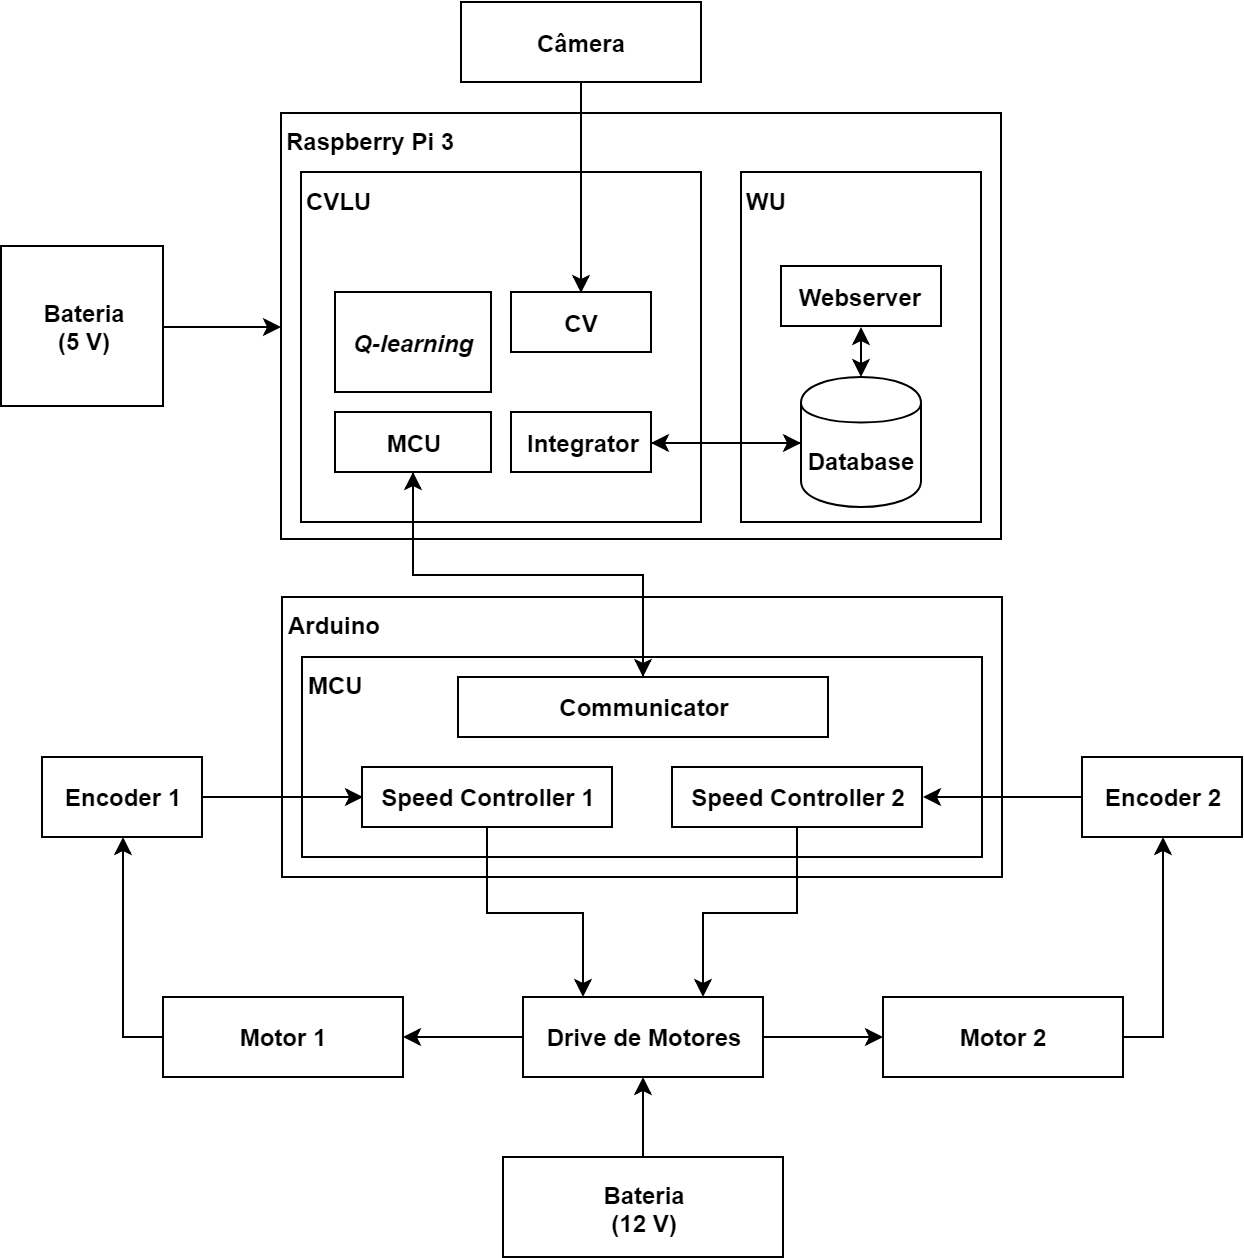
\includegraphics[scale=0.20]{Figuras/blockDiagramFull.png} 
\caption{Diagrama de blocos dos subsistemas implementado.}
\label{fig:blockDiagramFull}
\end{figure}

Alguns características devem ser consideradas na implementação de um abordagem de RL online, como o fato de ser praticamente impossível assumir que a observação do estado do agente é absoluta e livre de ruídos, uma vez que é obtida por sensores, tornando necessário o uso de filtros digitais como filtro Butterworth ou de média móvel. 

A Figura \ref{fig:alfFlux} mostra o fluxograma das principais operações realizadas durante as etapas de aquisição de conhecimento do ambiente e de consolidação do processo de aprendizado. 

\begin{figure}
\centering
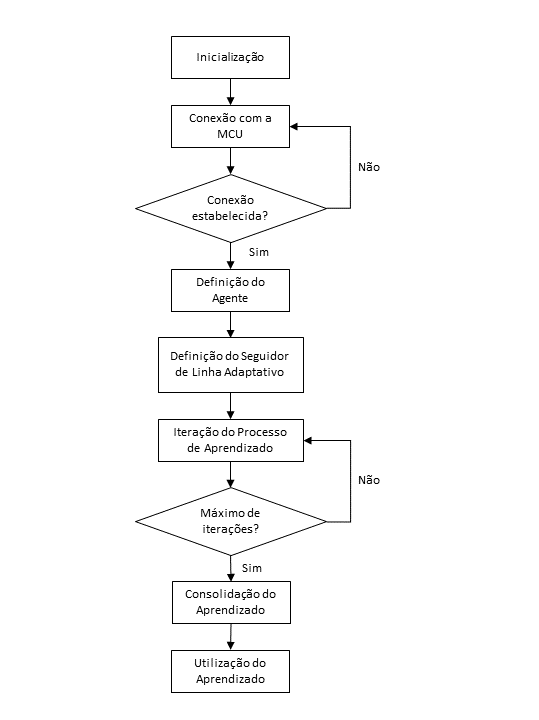
\includegraphics[scale=0.65]{Figuras/alfFlux2.png} 
\caption{Fluxograma de um ciclo básico de funcionamento implementado para o robô seguidor de linha adaptativo.}
 \label{fig:alfFlux}
\end{figure}

Inicialmente todas as variáveis como lista de estados, ações e recompensas são inicializadas conforme a configuração adotada para o processo. Em seguida, é feita uma tentativa de conexão com a MCU. Em caso de falha, novas tentativas são feitas até que seja obtido sucesso. Caso a conexão seja estabelecida com sucesso, o programa segue para o passo seguinte que consiste na definição das estruturas de dados necessárias para execução do programa que implementa o \textit{Q-learning} e Seguidor de Linha Adaptativo. Uma vez configurado, o processo de aprendizado é iniciado e permanece em execução até que todas as iterações sejam executadas, treinando o controlador de translação e orientação. Por fim ocorre a consolidação do aprendizado a partir do qual o robô passa a executar a política de ações aprendida no decorrer do aprendizado.

\subsection{Sistema de Visão Computacional}

Neste trabalho, um sistema de visão computacional é utilizado para identificar o caminho a ser seguido (estabelecido através de linhas no ambiente) e estimar o desvio de posição através da contagem dos pixels entre centro da linha e o centro da imagem. Se o centro da linha aparece à esquerda com relação ao centro da imagem, o robô encontra-se à direita da linha, caso contrário, o robô está a esquerda da linha. Para seguir a linha corretamente, o robô deve manter o centro com o menor desvio possível do centro da imagem captada pela câmera.  
A imagem obtida é cortada em uma região específica para otimizar o processamento. Em seguida, esta imagem é convertida para escala de cinza e um filtro Gaussiano é aplicado para diminuir o ruído após a conversão. Por fim, faz-se uma binarização da imagem, que transforma \textit{pixels} com valores acima de um limiar em branco e abaixo deste mesmo limiar em preto. Desta forma, basta identificar o polígono formado pela linha e o seu centro, que possui uma coordenada na horizontal e na vertical. Como o propósito é ver o quão alinhado o robô está em relação à linha demarcada, a coordenada horizontal é a mais relevante. Neste caso, o desvio pode ser determinado pela diferença entre as coordenadas horizontais do centro da linha e do centro da imagem. 

A Figura \ref{fig:cvuBlocks} contém um fluxograma do processamento de imagem e a Figura \ref{fig:im_proc_lf} ilustra como o cálculo do desvio é realizado.

\begin{figure}
\centering 
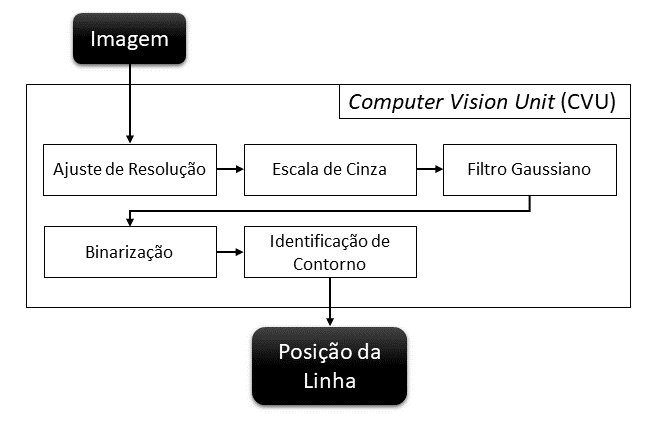
\includegraphics[scale=0.5]{Figuras/cvuBlocks2.png}
\caption{Fluxograma do processamento realizado para cada amostrade imagem.}
 \label{fig:cvuBlocks}
\end{figure}

\begin{figure}
\centering 
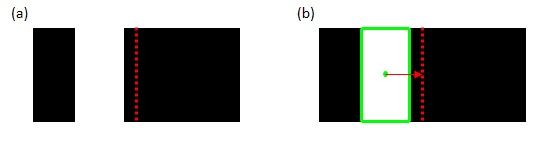
\includegraphics[scale=0.55]{Figuras/im_proc_lf.jpg} 
\caption{Processamento da imagem amostrada pela câmera da CVLU. (a) Amostragem, filtragem e binarização. (b) Cálculo do desvio.}
\label{fig:im_proc_lf}
\end{figure} 

%Este processo foi implementado por meio de dois métodos: \textit{processNewFrame()} e \textit{getLineCenter()}. A cada novo \textit{frame} obtido pela câmera, o primeiro método é chamado, aplicando todas as transformações na imagem. Na sequência, o segundo método é executado para obter a coordenada horizontal do centro da linha a partir do processamento realizado anteriormente. 

\subsection{Q-Learning Online}
A estratégia de RL, baseada no algoritmo \emph{Q-learning}, é proposta para derivar de forma online um controlador de 2-DoF para controlar o seguimento de caminho realizado pelo robô não-holonômico, considerando o acoplamento e a não-linearidade existe no sistema. Em cada iteração do algoritmo, o sistema de visão  estima o desvio do robô em relação ao caminho a ser percorrido e, em seguida, calcula o estado atual da plataforma. Logo depois, as ações são escolhidas com base nos valores da tabela Q e comandos são emitidos para a Unidade de Controle de Motores (MCU) executar as ações. Após o término da execução, o novo estado é estimado, a recompensa é calculada e a posição da tabela Q correspondente ao estado anterior e a ações escolhidas são atualizadas, \citep{qLearningDev}. 

A Figura \ref{fig:qlearningflux} contém um fluxograma das operações básicas executadas no contexto do processo do aprendizado. O processo acontece de forma cíclica sempre recomeçando pela determinação do estado atual.

\begin{figure}
\centering  
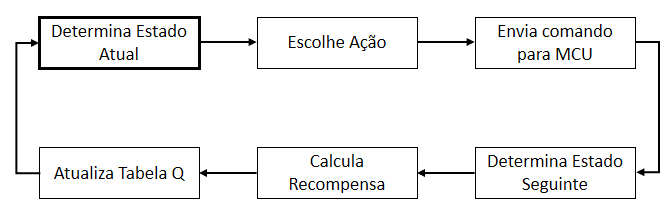
\includegraphics[scale=0.5]{Figuras/qlearningflux.png}
\caption{Fluxograma geral do algoritmo \textit{Q-learning} implementado.}
\label{fig:qlearningflux}
\end{figure} 

A determinação dos estados é feita com base na posição horizontal do centro da linha. Considere uma imagem com resolução $(w,h)$ \textit{pixels}, sendo $w$ a quantidade de \textit{pixels} na horizontal e $h$ a quantidade na vertical. Sendo assim, os possíveis valores de posição horizontal $x$ estão dentro do intervalo $[1,w]$ e $x = w/2$ é o centro da imagem. 

O intervalo $[1,w]$ é dividido em $n-1$ partes, onde $n$ é a quantidade de estados em que há $n-1$ estados onde é possível identificar a linha e $1$ estado onde a linha não está no campo de visão do robô. Cada estado é definido por um intervalo fechado $[s,f]$, onde $s$ indica o \textit{pixel} de início e $f$ o \textit{pixel} de término. A Figura \ref{fig:stateDefinitionSystem} contém uma ilustração que descreve a lógica de definição do estados do agente para um caso em que $w = 300$ e $n = 4$. 

Quando a linha encontra-se fora do campo de visão do robô, o método de processamento retorna o valor zero, caracterizando o estado onde o robô encontra-se sem referência de trajetória. Neste caso, ao fim do processo de aprendizado, o \textit{Q-learning} deverá selecionar a ação que fará com que o robô encontre novamente a linha. 

\begin{figure}
\centering
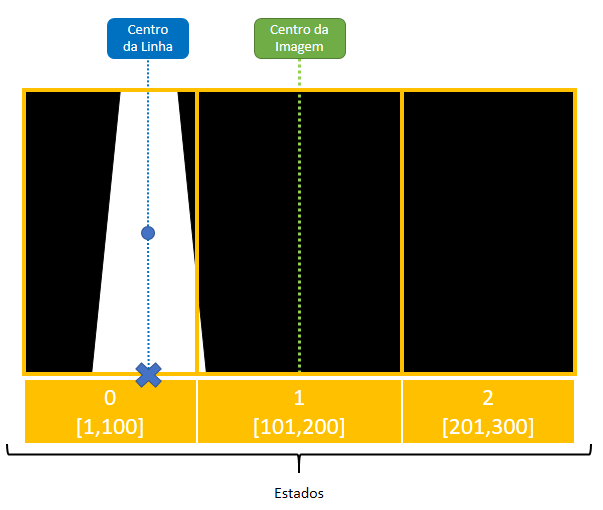
\includegraphics[scale=0.55]{Figuras/stateDefinitionSystem.png}
\caption{Delimitação dos estados para $w = 300$ e $n = 4$. O centro da linha encontra-se no intervalo correspondente ao estado 0.} 
\label{fig:stateDefinitionSystem}
\end{figure} 

Os pares $[s,f]$ são armazenados em uma lista no programa principal da CVLU, conforme pode ser observado na Tabela \ref{tab:statesOnMemory} que ilustra um exemplo em que $w = 300$ e $n = 4$.

\begin{table}
\centering
\ABNTEXfontereduzida
\caption{Lista que armazena as informações dos estados utilizados no \textit{Q-learning} considerando o caso de quatro estados.} \label{tab:statesOnMemory}
\begin{tabular}{cc}
Índice & Intervalos\\ \hline
0 & [1,100]\\ 
1 & [101,200]\\ 
2 & [201,300] \\ 
3 & [0,0]\\ \hline
\end{tabular}
\end{table}

Uma vez que o estado atual foi determinado, o programa segue para escolher a ação a ser tomada tomando como base a tabela Q. Uma probabilidade no intervalo fechado [0,1] é sorteada e a linha correspondente ao estado atual é percorrida enquanto o valor acumulado de probabilidade das possíveis ações seja menor do que a probabilidade sorteada. A escolha da ação se dá pela coluna da última posição acessada nesta varredura.

As ações, são definidas como pares de valores ${(rpm_1,rpm_2)}$, onde o primeiro valor representa a velocidade angular do motor 1 (esquerdo) e o segundo a velocidade do motor 2 (direito), ambas em rotações por minuto. No caso do robô seguidor de linha, é necessário haver pelo menos três ações: curva para esquerda, seguir em frente, curva para a direita. O número de ações impacta diretamente na forma de movimentação do robô nas curvas, pois é possível definir curvas e vários graus de intensidade com maiores quantidades de ações. A Tabela \ref{tab:basicActions} contém um exemplo de combinações de velocidades para as três ações básicas do robô seguidor de linha.

\begin{table}
\centering
\ABNTEXfontereduzida
\caption{Tabela ações básicas do agente.} \label{tab:basicActions}
\begin{tabular}{cccc}
Ação & Índice & Motor 1 & Motor 2\\ \hline 
Curva (Esquerda) & 0 & 0 rpm & 100 rpm\\ 
Seguir em Frente & 1 & 100 rpm & 100 rpm\\
Curva (Direita) & 2 & 100 rpm & 0 rpm\\ \hline
\end{tabular}
\end{table}

As configurações de cada uma das ações são armazenadas em uma lista onde o índice equivale a ação e o conteúdo à combinação de velocidades dos motores, conforme o exemplo contido na Tabela \ref{tab:intermediateActionsTab}, que mostra uma lista para o caso de cinco ações ações.

A CVLU e MCU foram implementados em hardwares distintos a fim de paralelizar a execução dos programas principais e garantir um melhor desempenho. Sendo assim, foi necessário criar um protocolo de comunicação padronizado entre os dois dispositivos para viabilizar que as ações calculadas pela CVLU fossem enviadas e executadas pela MCU.

Conforme mencionado anteriormente, para o robô conseguir seguir a linha, ele deve manter o centro da linha o mais próximo possível do centro da imagem. Sendo assim, o cálculo das recompensas é feito de tal modo que o estado que garante a maior recompensa é o que contém o centro da imagem. Quanto mais afastado do centro, menor a recompensa associada. A menor de todas as recompensas é associada ao estado onde a linha está fora do campo de visão do robô. Neste trabalho, optou-se por implementar o cálculo da recompensa através da associação direta entre o estado e o seu respectivo valor de recompensa, semelhante à lista de estados e ações. Entretanto, esse cálculo pode ser feito de outras formas, como por exemplo, utilizando uma função para calcular a recompensa de acordo com a distância entre o centro da linha e centro da imagem.

\begin{figure}
\centering  
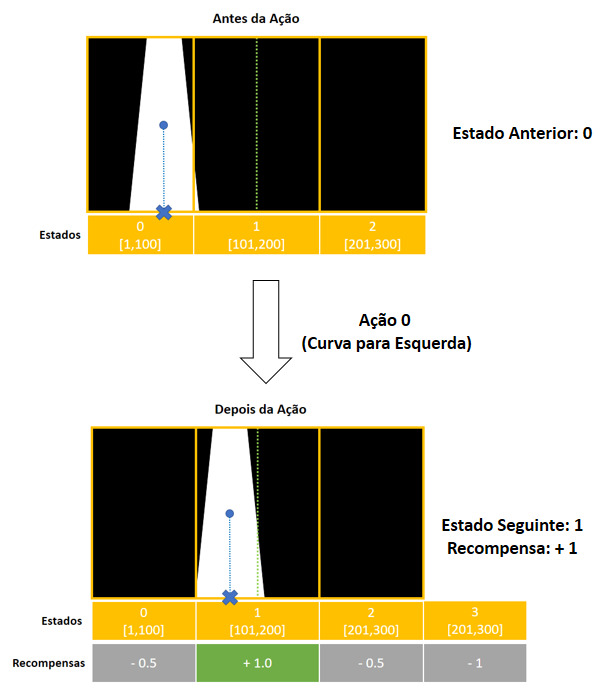
\includegraphics[scale=0.55]{Figuras/statesAndRewards.png}
\caption{Determinação do estado atual, escolha e execução da ação e determinação do estado seguinte.}
\label{fig:statesAndRewards}
\end{figure} 


Após o término das iterações, a CVLU faz um processo de consolidação da política obtida. A tabela Q do agente é varrida e um mapa é construído entre cada estado e a ação que possuir o maior valor acumulado ao término das iterações. Desta forma, ao invés de sempre realizar varreduras sobre a tabela Q, o robô pode utilizar a política aprendida num processo de aprendizado, consolidada na forma de um mapa estado-ação, de forma mais eficiente e concisa, eliminando iterações e varreduras desnecessárias.

%**************************************************************
% Seção 4
%************************************************************
\section{Resultados}

Os Estudos de Caso apresentados a seguir foram realizados em uma superfície escura cuja trajetória a ser seguida era definida por uma linha branca que descrevia um circuito fechado com curvas de aspectos variados.

\subsection{Estudo de Caso I}

O primeiro estudo de caso foi configurado  para contemplar o mínimo de estados possíveis e ações necessárias para a tarefa de seguir uma linha. Neste caso, o processo de aprendizado possuía quatro estados, com os quais seria possível distinguir posições como à esquerda da linha, à direita da linha, sobre a linha e sem visão da linha. 

Definiu-se um conjunto básico de três ações que incluíam movimentos de curva à esquerda, curva à direita e seguir em frente. A ação de ficar parado foi desconsiderada, pois, além de não promover uma mudança de estados, não faria com que o robô avançasse no circuito. Os estados e ações encontram-se descritos na Tabela \ref{tab:basicStatesTab} e na Tabela \ref{tab:basicActionsTab}, respectivamente. O processo de aprendizado foi configurado com $\alpha = 0,1$, $\lambda = 0,9$ e 2000 iterações. 

\begin{table}[htb]
\centering
\caption{Estados do Estudo de Caso I.} \label{tab:basicStatesTab}
\begin{tabular}{ccccc}
Estado & Descrição & Início & Fim & Recompensa\\ \hline
0 & Linha à Esquerda & 1 & 101 & -0,07\\
1 & Sobre a linha & 102 & 139 & 1,0\\ 
2 & Linha à Direita & 140 & 240 & -0,07\\
3 & Sem visão da linha  & 0 & 0 & -1,0\\ \hline
\end{tabular}
\end{table}

\begin{table}[htb]
\centering
\caption{Ações do Estudo de Caso I.} \label{tab:basicActionsTab}
\begin{tabular}{cccc}
Ação & Descrição & Motor 1 & Motor 2\\ \hline
0 & Curva à Esquerda & 0 & 100 rpm\\ 
1 & Seguir em Frente & 100 rpm & 100 rpm\\ 
2 & Curva à Direita & 100 rpm & 0\\ \hline
\end{tabular}
\end{table}

A Figura \ref{fig:basic_chart1} contém o gráfico dos valores finais dos pares estado-ação para cada um dos estado. Considerando o Estado 0, em que a linha encontra-se a esquerda do robô, o par de maior valor foi (Estado 0, Ação 0), o que significa que o robô aprendeu que, se a linha encontra-se a sua esquerda, ele deve fazer uma curva à esquerda. O foi observado para o Estado 1 e Estado 2, em que os pares de maiores valores são (Estado 1, Ação 1) e (Estado 2, Ação 2), respectivamente. 

Considerando o Estado 3, o maior valor está associado ao par (Estado 3, Ação 2), significando que o robô aprendeu que a melhor ação é executar uma curva à direita em caso de perder a referência da linha. Também é possível inferir que a ação de seguir em frente seria a pior opção, pois a ação de menor valor acumulado. 

\begin{figure}
\centering 
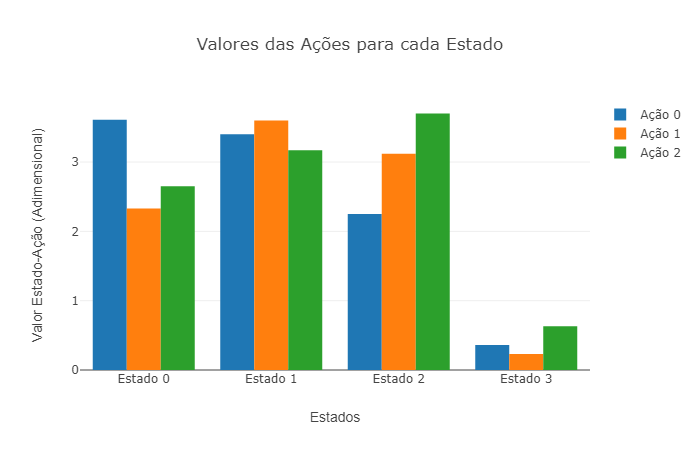
\includegraphics[scale=0.35]{Figuras/basic_chart1.png}
\caption{Valores finais (adimensionais) dos pares estado-ação para cada estado em função da ação no Estudo de Caso I.} 
\label{fig:basic_chart1}
\end{figure}

A evolução da Recompensa Média Acumulada ao longo das iterações encontra-se na Figura \ref{fig:basic_chart2}. É possível notar que este gráfico apresenta uma tendência em convergir para um valor constante no decorrer das iterações, indicando a convergência do método. 

\begin{figure}
\centering 
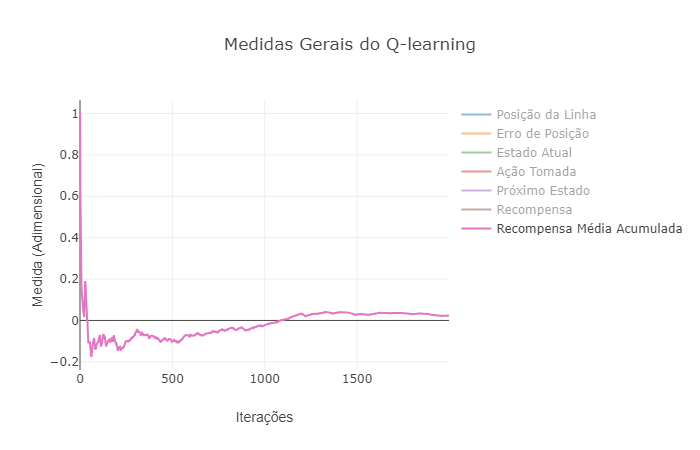
\includegraphics[scale=0.35]{Figuras/basic_chart2.png}
\caption{Recompensa Média Acumulada ao longo das iterações no Estudo de Caso I.} 
\label{fig:basic_chart2}
\end{figure}

A Figura \ref{fig:basic_chart3} contém um Mapa de Calor, que indica a quantidade de vezes que cada par estado-ação foi utilizado acessado ao longo do processo. Nele é possível observar que os pares que tiveram o maior valor associado possuíam mais acessos, exceto no caso do Estado 3. Com este mapa de calor, obteve-se a Tabela \ref{tab:accessPercent}, que mostra o percentual de acesso para cada par de maior valor associado. 

\begin{figure}
\centering 
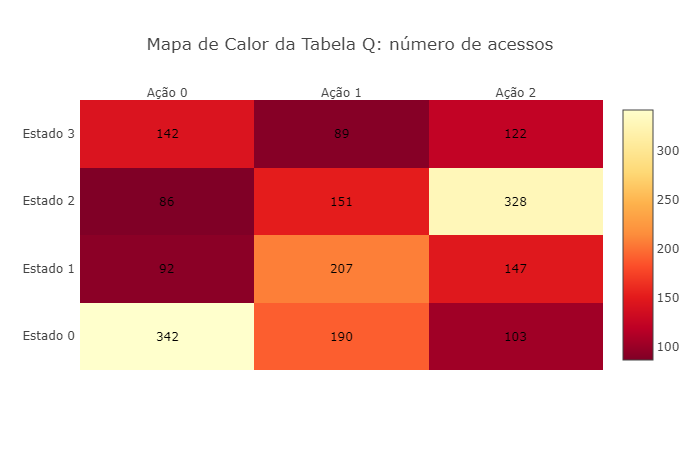
\includegraphics[scale=0.35]{Figuras/basic_chart3.png}
\caption{Mapa de Calor da quantidade de acesso aos pares estado-ação relativo ao Estudo de Caso I.} 
\label{fig:basic_chart3}
\end{figure}

\begin{table}
\centering
\caption{Percentual de acessos dos pares estado-ação de maior valor no Estudo de Caso I.} \label{tab:accessPercent}
\begin{tabular}{ccccc}
\thead{Estado\\ } & \thead{Total de \\Acessos} & \thead{Ação com \\Maior Valor} & \thead{Acessos \\da Ação} & \thead{Percentual}\\ \hline
0 & 635 & Ação 0 & 342 & 53,8 \%\\
1 & 446 & Ação 1 & 207 & 46,4 \%\\
2 & 565 & Ação 2 & 328 & 58,1 \%\\
3 & 353 & Ação 2 & 122 & 34,6 \%\\\hline
\end{tabular}
\end{table}

\subsection{Estudo de Caso II}

O objetivo deste Estudo de Caso foi avaliar se o método ainda seria capaz de definir um controlador adequado para um maior número de estados e ações, bem como observar os efeitos dessas mudanças de configuração. O processo de aprendizado foi configurado com seis estados e cinco ações. Pelos mesmos motivos mencionados anteriormente, a ação de ficar parado foi desconsiderada. 

Os estados e suas respectivas recompensas encontra-se na Tabela \ref{tab:intermediateStatesTab}, enquanto as ações estão descritas na Tabela \ref{tab:intermediateActionsTab}. Este processo foi configurado utilizando $\alpha = 0,1$, $\lambda = 0,9$, 3000 iterações e durou cerca de 35 minutos.

\begin{table}
\centering
\caption{Estados do Estudo de Caso} \label{tab:intermediateStatesTab}
\begin{tabular}{ccccc}
Estado & Posição da Linha & Início & Fim & Recompensa\\ \hline
0 & Extrema Esquerda & 1 & 61 & -0,05 \\ 
1 & Esquerda & 62 & 100 & -0,02 \\
2 & Sobre a linha & 101 & 140 & 1,0\\
3 & Direita & 141 & 179 & -0,02\\
4 & Extrema Direita & 180 & 240 & -0,05\\
5 & Sem visão (perdido) & 0 & 0 & -1,0\\ \hline
\end{tabular}
\end{table}

\begin{table}
\centering
\caption{Ações do Estudo de Caso.} \label{tab:intermediateActionsTab}
\begin{tabular}{cccc}
Ação & Descrição & Motor 1 & Motor 2\\ \hline
0 & Giro anti-horário & -100 rpm & 100 rpm\\ 
1 & Curva à Esquerda & 0 & 100 rpm\\ 
2 & Seguir em frente & 100 rpm & 100 rpm \\
3 & Curva à Direita & 100 rpm & 0\\
4 & Giro horário & 100 rpm & -100 rpm\\ \hline
\end{tabular}
\end{table}

Os valores finais dos pares estado-ação para cada um dos estados encontram-se ilustrados no gráfico da Figura \ref{fig:enhanced_chart1}. Considerando o Estado 0 e o Estado 4, é possível observar que os pares de maior valor são (Estado 0, Ação 0) e (Estado 4, Ação 4), indicando que após o processo de aprendizado, o robô aprendeu que para os desvios mais acentuados deve tomar as ações correspondentes às curvas mais bruscas. 

Analogamente, o mesmo pode ser observado para o Estados 1 e Estado 3, em que o robô apresenta um leve desvio de posição. Nestes casos, os pares de maior valor são (Estado 1, Ação 1) e (Estado 3, Ação 3), indicando que após o processo de aprendizado, o robô aprendeu que as ações correspondentes às curvas mais suaves são mais adequadas para desvios menos acentuados.

\begin{figure}
\centering 
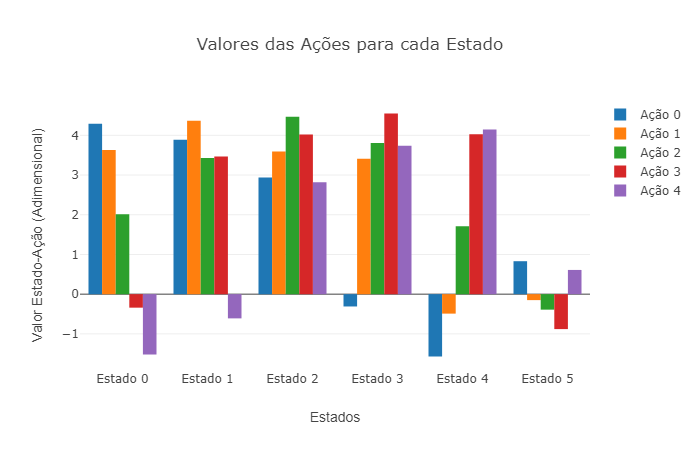
\includegraphics[scale=0.35]{Figuras/enhanced_chart1.png}
\caption{Valores estado-ação (adimensionais) para cada estado em função da ação no Estudo de Caso II.} \label{fig:enhanced_chart1}
\end{figure}

Um fato interessante a se destacar foi o resultado obtido para o Estado 5 em que os dois pares de maior valor obtidos foram (Estado 5, Ação 0) e (Estado 5, Ação 4), tornando possível inferir que o robô aprendeu que curvas bruscas o fazem retornar à linha de forma mais eficiente do que curvas suaves quando encontra-se perdido. 

A Recompensa Média Acumulada ao longo das iterações encontra-se no gráfico da Figura \ref{fig:enhanced_chart2} e também possui uma tendência em convergir para um valor à medida que as iterações avançam. Entretanto, quando comparado ao Estudo de Caso I, a taxa de convergência ao longo das iterações é menor, o que indica que o número de iterações necessárias para que a Recompensa Média Acumulada comece a convergir também aumenta.

Ao aumentar o número de estados e ações é possível tornar o controlador mais preciso, uma vez que possibilita aumentar a variedade de tipos de curvas e distinção de estados. Entretanto isso faz com que a Matriz Q aumente de tamanho, o que aumenta a complexidade computacional do algoritmo. Isso se evidencia pela necessidade de mais iterações como observado no Estudo de Caso II.

\begin{figure}
\centering 
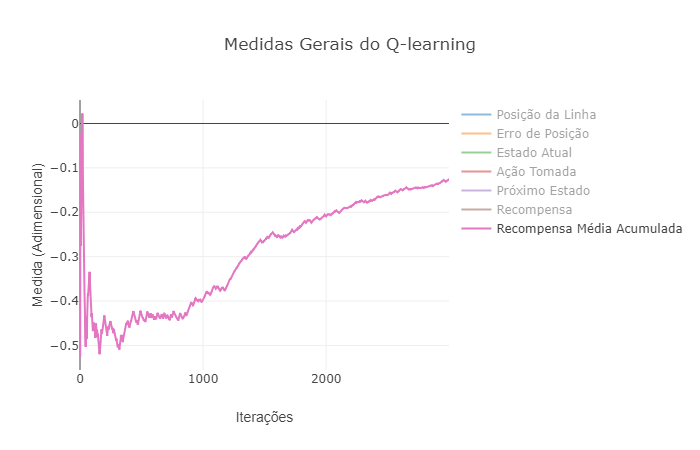
\includegraphics[scale=0.35]{Figuras/enhanced_chart2.png}
\caption{Recompensa média acumulada ao longo das iterações no Estudo de Caso 2.} \label{fig:enhanced_chart2}
\end{figure}

O mapa de calor da Figura \ref{fig:enhanced_chart3} mostra o número de acessos de cada um dos pares estado-ação neste estudo de caso. Neste mapa é possível observar que os pares de maior valor associado foram os mais acessados.A partir deste resultado, pode-se obter a Figura \ref{tab:accessPercentEnhanced}, que apresenta o percentual de acesso aos pares de maior valor para cada estado. Outro fato que se repetiu diz respeito ao Estado 5, em que a linha estava fora do campo de visão: o par com maior valor associado não foi o mais acessado.

\begin{figure}
\centering 
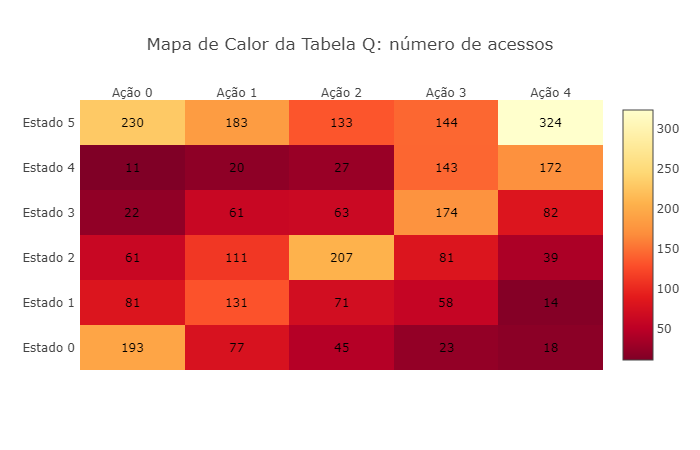
\includegraphics[scale=0.35]{Figuras/enhanced_chart3.png}
\caption{Mapa de Calor da quantidade de acesso aos pares estado-ação relativo ao Estudo de Caso 2.} \label{fig:enhanced_chart3}
\end{figure}

\begin{table}[htb]
\centering
\caption{Percentual de acessos dos pares estado-ação de maior valor no Estudo de Caso.} \label{tab:accessPercentEnhanced}
\begin{tabular}{ccccc}
\thead{Estado\\ } & \thead{Total de \\Acessos} & \thead{Ação com \\Maior Valor} & \thead{Acessos \\da Ação} & \thead{Percentual}\\ \hline
0 & 356 & Ação 0 & 193 & 54,2 \%\\
1 & 355 & Ação 1 & 131 & 36,9 \%\\
2 & 499 & Ação 2 & 207 & 41,5 \%\\
3 & 402 & Ação 3 & 174 & 43,3 \%\\
4 & 373 & Ação 4 & 172 & 46,1 \%\\
5 & 1014 & Ação 0 & 230 & 22,7 \%\\\hline
\end{tabular}
\end{table}

A partir dos resultados apresentados pode notar que o controlador aprendido foi capaz de realizar o seguimento de caminho de forma eficiente. 

Além de possuir a capacidade de executar curvas mais fechadas devido à adição das ações de girar sobre o próprio eixo, o robô é capaz de retornar mais rapidamente à pista.

\section{Conclusão}

A partir dos estudos de casos apresentados, foi possível observar que a abordagem utilizada conseguiu derivar controladores capazes de fazer o robô seguir a trajetória definida por uma linha da forma esperada em ambos os casos. Estes estudos também mostraram que existe uma relação entre a quantidade de estados, ações e o número de iterações necessárias para que a Recompensa Média Acumulada convirja. Quanto maior o número de estados e ações, maior é a quantidade de iterações necessárias. Este resultado faz sentido, pois o tamanho da matriz Q aumenta, o que demanda uma maior quantidade de iterações para que seja varrida adequadamente. 

Um outro resultado interessante é que a política aprendida no Estudo de Caso II mostrou que o robô aprendeu a escolher executar curvas mais bruscas quando estava sem visão da trajetória. Na prática, esta ação garante que o robô encontre novamente o trajeto mais rapidamente, em menos iterações e com menos punições, maximizando a recompensa.

\bibliography{ifacconf}             % bib file to produce the bibliography
                                                     % with bibtex (preferred)
                                                   
%\begin{thebibliography}{xx}  % you can also add the bibliography by hand

%\bibitem[Able(1956)]{Abl:56}
%B.C. Able.
%\newblock Nucleic acid content of microscope.
%\newblock \emph{Nature}, 135:\penalty0 7--9, 1956.

%\bibitem[Able et~al.(1954)Able, Tagg, and Rush]{AbTaRu:54}
%B.C. Able, R.A. Tagg, and M.~Rush.
%\newblock Enzyme-catalyzed cellular transanimations.
%\newblock In A.F. Round, editor, \emph{Advances in Enzymology}, volume~2, pages
%  125--247. Academic Press, New York, 3rd edition, 1954.

%\bibitem[Keohane(1958)]{Keo:58}
%R.~Keohane.
%\newblock \emph{Power and Interdependence: World Politics in Transitions}.
%\newblock Little, Brown \& Co., Boston, 1958.

%\bibitem[Powers(1985)]{Pow:85}
%T.~Powers.
%\newblock Is there a way out?
%\newblock \emph{Harpers}, pages 35--47, June 1985.

%\bibitem[Soukhanov(1992)]{Heritage:92}
%A.~H. Soukhanov, editor.
%\newblock \emph{{The American Heritage. Dictionary of the American Language}}.
%\newblock Houghton Mifflin Company, 1992.

%\end{thebibliography}

\end{document}
